\documentclass[12pt,a4paper]{article}%
\usepackage[]{graphicx}\usepackage[]{color}
%% maxwidth is the original width if it is less than linewidth
%% otherwise use linewidth (to make sure the graphics do not exceed the margin)

%2multibyte Version: 5.50.0.2960 CodePage: 1252
\usepackage{amsfonts}
\usepackage{amssymb}
\usepackage[centertags]{amsmath}
\usepackage{graphicx}%
\usepackage{natbib}
\usepackage{color}
\usepackage[dvipsnames,svgnames*]{xcolor}
\usepackage{array}
\usepackage[hidelinks]{hyperref}
\usepackage[font=small,skip=5pt]{caption}
\usepackage[aboveskip=2pt]{subcaption}
\usepackage{amsmath}
\usepackage[]{algorithm2e}
\usepackage{amsthm}
%\usepackage{tikz}
%\usetikzlibrary{bayesnet}
\usepackage{url}
\usepackage{wasysym}
\usepackage{ulem}
\usepackage{afterpage}
\usepackage{bbm}
\setcounter{MaxMatrixCols}{30}
\providecommand{\U}[1]{\protect\rule{.1in}{.1in}}
\newtheorem{theorem}{Theorem}
\newtheorem{acknowledgement}[theorem]{Acknowledgement}
\newtheorem{axiom}[theorem]{Axiom}
\newtheorem{case}[theorem]{Case}
\newtheorem{claim}[theorem]{Claim}
\newtheorem{conclusion}[theorem]{Conclusion}
\newtheorem{condition}[theorem]{Condition}
\newtheorem{conjecture}[theorem]{Conjecture}
\newtheorem{corollary}[theorem]{Corollary}
\newtheorem{criterion}[theorem]{Criterion}
\newtheorem{definition}[theorem]{Definition}
\newtheorem{example}[theorem]{Example}
\newtheorem{exercise}[theorem]{Exercise}
\newtheorem{lemma}[theorem]{Lemma}
\newtheorem{notation}[theorem]{Notation}
\newtheorem{problem}[theorem]{Problem}
\newtheorem{proposition}[theorem]{Proposition}
\newtheorem{remark}[theorem]{Remark}
\newtheorem{solution}[theorem]{Solution}
\newtheorem{summary}[theorem]{Summary}
\setlength{\topmargin}{0in}
\setlength{\oddsidemargin}{0.1in}
\setlength{\evensidemargin}{0.1in}
\setlength{\textwidth}{6.5in}
\setlength{\textheight}{8.25in}
\numberwithin{equation}{section}
\title{MCMC Informed Variational Bayes}
\author{Nathaniel Tomasetti, Catherine Forbes and Anastasios Panagiotelis}
\date{}
\begin{document}

\maketitle

\tableofcontents

\section{Introduction}
\label{Intro}

Consider a high frequency time series with observed values $y_{1}, \dots, y_{T+S}$, collectively denoted by $y_{1:T+S}$, with a forecaster interested in the forecast distribution of the future value $y_{T+S+h}$, where $S \geq 1$.  

Many time series models of interest contain a set of global parameters $\boldsymbol{\theta}$ and observation specific latent variables $x_{0:T}$, such that $x_t$ is assumed to follow a Markovian structure and $y_t$ is conditionally independent of $y_{1:t-1}$, given $\boldsymbol{\theta}$ and $x_t$. One of the most common computational techniques for models with latent states is Markov Chain Monte Carlo (MCMC), which involves iterative sampling from a Markov Chain designed to converge to the true posterior distribution, however these approaches can have slow convergence rates as they generally do not admit parallel processing or data subsampling to speed up computation. In this paper it is assumed that an MCMC sample of $p(\boldsymbol{\theta}, x_{0:T} | y_{1:T})$ is available at time $T+S$, but the convergence of the required MCMC algorithm is slow, so a posterior distribution conditioned on any additional observations of $y_t, t = T+1, \dots, T+S$ will not be available before observation of $y_{T+S+h}$. 

With $p(\boldsymbol{\theta}, x_{0:T}| y_{1:T})$ available, the forecast distribution of $p(y_{T+S+h} | y_{T})$ is obtainable to make an $S+h$ step ahead forecast of $y_{T+S+h}$. However, it is desirable to incorporate the information contained in realisations of $y_{T+1:T+S}$ to obtain $p(y_{T+S+h} | y_{T+S})$, which should provide a forecast with reduced uncertainty due to the smaller forecast horizon of $h$ steps. If certain model restrictions are met, $y_{T+1:T+S}$ can be included in the forecast by using filtering techniques such as the Kalman filter or particle filter. If these restrictions are not met, or the filtering technique is too computationally intensive to perform before $T+S+h$, then the forecaster is unable to obtain $p(y_{T+S+h} | y_{T+S})$. 

An alternative to MCMC is Variational Bayes (VB), which approximates the posterior distribution with a tractable alternative denoted by $q$, optimising the parameters of this approximation so that the approximation is close by some metric to the actual posterior. A VB optimisation algorithm is often orders of magnitude faster than MCMC, with the application of parallel processing and data subsampling available to scale compuation to large datasets. With the use of VB the approximate posterior $q(\boldsymbol{\theta}, x_{0:T+S} | y_{1:T+S})$ is available before $T+S+h$, and thus the approximate forecast distribution $q(y_{T+S+h} | y_{T+S})$ can be used.

Variational Bayes involves an implicit trade-off: reducing the forecast horizon of $y_{T+S+h}$ from $S+h$ to $h$ reduces the uncertainty of the forecast, but the approximation will increase the statistical error. This paper explores that trade-off for a Dynamic Linear Model and a Stochastic Volatility Model, two common latent state time series models, and introduces MCMC Informed Variational Bayes (MIVB), which emphasises the use of information available in MCMC samples of $p(\boldsymbol{\theta}, x_{0:T} | y_{1:T+S})$ as an alternative to standard `black box' approaches where a generic functional form is used for all models.

\begin{itemize}
\item Section Two: Variational Bayes, Optimisation and ADVI
\item Section Three: MCMC Informed Variational Bayes
\item Section Four: Simulation results for DLM, SVM
\item Section Five: Empirical SVM
\item Section Six: Discussion
\end{itemize}

\section{Variational Bayes}
\label{VB}
Variational Bayes posits a divergence function between the true posterior distribution $p(\boldsymbol{\theta}, x_{1:T+S} | y_{1:T+S})$ and some approximating distribution $q(\boldsymbol{\theta}, x_{1:T+S} | \boldsymbol{\lambda})$, choosing the parameters $\boldsymbol{\lambda}$ for a given functional form $q$ that minimises the divergence function. The notation for $q$ supresses the dependence of the distribution on $y_{1:T+S}$ as $\boldsymbol{\lambda}$ is typically a function of $y_{1:T+S}$.

This paper will follow the traditional approach, where the divergence function is the Kullback-Leibler (KL) divergence (Kullback and Leibler, 1951) from $q(\boldsymbol{\theta}, x_{1:T+S}| \boldsymbol{\lambda})$ to the true posterior $p(\boldsymbol{\theta}, x_{1:T+S} | y_{1:T+S})$. The KL divergence is defined by
\begin{align}
\label{KL-def}
KL[q(\boldsymbol{\theta}, x_{1:T+S}| \boldsymbol{\lambda})\hspace{.1cm}||\hspace{.1cm}p(\boldsymbol{\theta}, x_{1:T+S} | y_{1:T+S})] &= \nonumber \\
\int q(\boldsymbol{\theta}, x_{1:T+S} | \boldsymbol{\lambda}) &\ln \left( \frac{q(\boldsymbol{\theta}, x_{1:T+S} | \boldsymbol{\lambda})}{p(\boldsymbol{\theta}, x_{1:T+S} |y_{1:T+S})}\right) d\boldsymbol{\theta} dx_{1:T+S}
\end{align}
and can alternatively be expressed as
\begin{equation}
\label{KL-ELBO}
KL[q(\boldsymbol{\theta}, x_{1:T+S} | \boldsymbol{\lambda})\hspace{.1cm}||\hspace{.1cm}p(\boldsymbol{\theta}, x_{1:T+S} | y_{1:T+S})] = \ln(p(y_{1:T+S})) - \mathcal{L}(q(\boldsymbol{\theta}, x_{1:T+S} | \boldsymbol{\lambda}), y_{1:T+S})
\end{equation}
where $\mathcal{L}(q(\boldsymbol{\theta}, x_{1:T+S} | \boldsymbol{\lambda}), y_{1:T+S})$ is referred to as the Evidence Lower Bound (ELBO), as it provides a lower bound on the unknown constant $\ln(p(y_{1:T+S}))$.  $\mathcal{L}(q(\boldsymbol{\theta}, x_{1:T+S} | \boldsymbol{\lambda}), y_{1:T+S})$ is defined by
\begin{equation}
\label{ELBO}
\mathcal{L}(q(\boldsymbol{\theta}, x_{1:T+S} | \boldsymbol{\lambda}), y_{1:T+S}) = \int q(\boldsymbol{\theta}, x_{1:T+S} | \boldsymbol{\lambda}) \ln \left( \frac{p(y_{1:T+S},\boldsymbol{\theta}, x_{1:T+S})}{q(\boldsymbol{\theta}, x_{1:T+S} | \boldsymbol{\lambda})} \right) d\boldsymbol{\theta}dx_{1:T+S},
\end{equation}
and as $\ln(p(y_{1:T+S}))$ is constant with respect to $\boldsymbol{\lambda}$, maximising (\ref{ELBO}) with respect to $\boldsymbol{\lambda}$ is equivalent to minimising (\ref{KL-def}). 

\subsection{ELBO Optimisation}
Equation (\ref{ELBO}) can be maximised using a gradient ascent approach, where the following update step is iteratively applied until (\ref{ELBO}) converges within some pre-specified tolerance:
\begin{equation}
\label{GradAscent}
\boldsymbol{\lambda}^{(m+1)} = \boldsymbol{\lambda}^{(m)} + \rho^{(m)} \frac{\delta}{\delta\boldsymbol{\lambda}} \mathcal{L}(q(\boldsymbol{\theta}, x_{1:T+S} | \boldsymbol{\lambda}^{(m)}), y_{1:T+S}).
\end{equation}
$\delta/\delta\boldsymbol{\lambda}\mathcal{L}(q(\boldsymbol{\theta}, x_{1:T+S} | \boldsymbol{\lambda}^{(m)}), y_{1:T+S})$ is the vector of partial derivatives of $\mathcal{L}(q(\boldsymbol{\theta}, x_{1:T+S} | \boldsymbol{\lambda}^{(m)}), y_{1:T+S})$ with respect to each element of $\boldsymbol{\lambda}$ evaluated at $\boldsymbol{\lambda}^{(m)}$. This update requires some initial values $\boldsymbol{\lambda}^{(0)}$ and a sequence $\rho^{(m)}, m = 1, 2, \dots$ known as the learning rate. If $\rho^{(m)}$ is chosen to satisfy the following conditions the algorithm is guaranteed to converge to a local maximum (Robbins and Munro, 1951).
\begin{align}
&\sum_{m=1}^{\infty} \rho^{(m)} =  \infty \\
&\sum_{m=1}^{\infty} (\rho^{(m)})^2 <  \infty.
\end{align}

Ranganath, Gerrish and Blei (2014) showed that a Monte Carlo estimate of the derivative of the ELBO can be given by
\begin{equation}
\label{ScoreDeriv}
\frac{\delta}{\delta\boldsymbol{\lambda}}\mathcal{L}(q(\boldsymbol{\theta}, x_{1:T+S} | \boldsymbol{\lambda}^{(m)}), y_{1:T+S}) \approx \frac{1}{N}\sum_{i=1}^{N} \frac{\delta}{\delta\boldsymbol{\lambda}} [\ln(q(\boldsymbol{\theta}_i, x_{1:T, i} | \boldsymbol{\lambda}^{(m)}))] \ln \left(\frac{p(y_{1:T+S}, \boldsymbol{\theta}_i, x_{1:T, i})}{q(\boldsymbol{\theta}_i, x_{1:T, i} | \boldsymbol{\lambda}^{(m)})} \right) 
\end{equation}
where $i = 1, \dots, N$ indicates simulations from $q(\boldsymbol{\theta}, x_{1:T+S} | \boldsymbol{\lambda}^{(m)})$. 
The terms in the sum in (\ref{ScoreDeriv}) can have large variances, and in practice a large value of $N$ is required to ensure a precise estimate of the gradient of the ELBO is obtained, slowing computation. 

The variance can be reduced by the reparameterisation trick of Kingma and Welling (2014), which introduces parameter free noise variables $\boldsymbol{\epsilon}$ and a differentiable transform $f$ such that
\begin{equation}
\label{Reparam}
\boldsymbol{\theta}, x_{1:T+S} = f(\boldsymbol{\epsilon}, \boldsymbol{\lambda}).
\end{equation}
Kingma and Welling (2014) show that an $f$ exists to transform $\boldsymbol{\epsilon}$ to any continuous random variable, with examples including a location-scale transform of a standard normal noise variable and an inverse-CDF transform of a uniform noise variable. Applying the transformation to $q(\boldsymbol{\theta}, x_{1:T+S} | \boldsymbol{\lambda})$ results in
\begin{equation}
\label{changevar}
q_{\epsilon}(\boldsymbol{\epsilon}) = q_{\theta, x}(f (\boldsymbol{\epsilon}, \boldsymbol{\lambda})) |J|
\end{equation}
where $J = d\boldsymbol{\theta}dx_{1:T+S}/d\boldsymbol{\epsilon}$ is the Jacobian Matrix of the transformation $f$. Substituting (\ref{changevar}) into (\ref{ELBO}) gives
\begin{align}
\mathcal{L}(q(\boldsymbol{\theta}, x_{1:T+S} | \boldsymbol{\lambda}), y_{1:T+S}) &= \int q_{\theta, x}(\boldsymbol{\theta}, x_{1:T+S} | \boldsymbol{\lambda}) \ln \left( \frac{p(y_{1:T+S},\boldsymbol{\theta}, x_{1:T+S})}{q_{\theta, x}(\boldsymbol{\theta}, x_{1:T+S} | \boldsymbol{\lambda})} \right) d\boldsymbol{\theta}dx_{1:T+S} \nonumber \\
&= \int q_{\epsilon}(\boldsymbol{\epsilon})|J|^{-1} \ln \left( \frac{p(y_{1:T+S},f (\boldsymbol{\epsilon}, \boldsymbol{\lambda}))}{q_{\epsilon}(\boldsymbol{\epsilon})|J|^{-1}} \right) d\boldsymbol{\theta}dx_{1:T+S} \nonumber \\
&= \int q_{\epsilon}(\boldsymbol{\epsilon}) \ln \left( \frac{p(y_{1:T+S},f (\boldsymbol{\epsilon}, \boldsymbol{\lambda}))}{q_{\epsilon}(\boldsymbol{\epsilon})|J|^{-1}} \right) d\boldsymbol{\epsilon} \nonumber \\
&= \int q_{\epsilon}(\boldsymbol{\epsilon}) \left( \ln (p(y_{1:T+S},f (\boldsymbol{\epsilon}, \boldsymbol{\lambda}))) - \ln(q_{\epsilon}(\boldsymbol{\epsilon})) + \ln(|J|)\right) d\boldsymbol{\epsilon}\nonumber \\
&= \mathcal{L}(q(\boldsymbol{\epsilon}), \boldsymbol{\lambda}, y_{1:T+S}). \label{reparamELBO}
\end{align}

The derivative of (\ref{reparamELBO}) can be estimated by
\begin{equation}
\label{ReparamDeriv}
\frac{\delta}{\delta\boldsymbol{\lambda}}\mathcal{L}(q(\boldsymbol{\epsilon}), \boldsymbol{\lambda}^{(m)}, y_{1:T+S}) \approx \frac{1}{N}\sum_{i=1}^{N} \frac{\delta}{\delta\boldsymbol{\lambda}} \left( \ln (p(y_{1:T+S}, f(\boldsymbol{\lambda}^{(m)}, \boldsymbol{\epsilon}_i))) + \ln(|J(\boldsymbol{\lambda}^{(m)}, \boldsymbol{\epsilon}_i)|) \right),
\end{equation}
where simulations of $\boldsymbol{\theta}$ and $x_{1:T+S}$ are replaced by simulations of $\boldsymbol{\epsilon}$ from $q(\boldsymbol{\epsilon})$. The variance of the terms in the sum of this estimator is often orders of magnitude lower than the estimator in (\ref{ScoreDeriv}); often $N = 1$ provides a precise enough estimate of the gradient for fast convergence.

\subsection{$q$ Functional Form}
A key decision in Variational Bayes is the choice of the functional form of the approximating distribution $q$. Much of the literature focuses on a `black box' functional form, where the same $q$ can be applied to many models. One popular black box method is Automatic Differentation Variational Bayes (ADVI, Kucukeliber, Ranganath, Gelman, Blei 2015; Kucukeliber, Tran, Ranganath, Gelman, Blei 2016), which first transforms each parameter $\theta$ and latent variable $x_t$ to the real line then selects a multivariate normal $q$ to approximate the posterior distribution of the transformed parameters with either a diagonal or non-diagonal covariance matrix.  

For illustration, consider a common latent variable time series model, the Dynamic Linear Model, described by (\ref{DLM:Measure}) and (\ref{DLM:Transition}).
\begin{align}
y_t &= \gamma + x_t + \sigma_y \epsilon_t \label{DLM:Measure}\\
x_t &= \phi x_{t-1} + \sigma_x \nu_t \label{DLM:Transition}
\end{align}
where $\epsilon_t$ and $\nu_t$ are independent $\mathcal{N}(0, 1)$ random variables. The priors used are
\begin{align}
\gamma &\sim \mathcal{N}(\bar{\gamma}, \sigma^2_{\gamma}) \\
\phi &\sim \mathcal{U}(-1, 1) \\
\sigma^2_y &\sim \mathcal{IG}(\mbox{shape = }\alpha_y, \mbox{scale = }\beta_y) \\
\sigma^2_x &\sim \mathcal{IG}(\mbox{shape = }\alpha_x, \mbox{scale = }\beta_x) \\
x_0 &\sim \mathcal{N}(0, \sigma^2_x(1 - \phi^2)^{-1})
\end{align}
where $\mathcal{IG}(\mbox{shape}, \mbox{ scale})$ denotes the inverse of a Gamma (shape, rate) distribution. Conjugate priors are chosen for $\gamma, \sigma^2_y$ and $\sigma^2_x$, while the uniform prior for $\phi$ constrains $p(\phi | y_{1:T+S})$ to have zero probability mass outside of the AR(1) stationary region. $\sigma^2_y$ and $\sigma^2_x$ are log-transformed such that $\theta^* = \{\gamma, \phi, \ln(\sigma^2_y), \ln(\sigma^2_x), x_{0:T}\} \in \mathbb{R}^{T+5}$. $100$ data sets $y_{1:T+S}$ are simulated for each $T \in \{50, 100, 250, 500, 1000, 2000, 5000, 10000\}$, using true parameter values of $\gamma = 2, \phi = 0.95, \sigma^2_y = 1$ and $\sigma^2_x=1$, and hyperparameters $\bar{\gamma} = 0, \sigma^2_{\gamma} = 10, \alpha_y = 1, \beta_y = 1, \alpha_x = 1$ and $\beta_x = 1$. For each case MCMC and ADVI are applied with both a diagonal and non-diagonal covariance matrix for $q(\theta^* | \boldsymbol{\lambda})$; however the non-diagonal version is not used for $T \geq 1000$ as the number of covariance parameters is quadratic in $T$. MCMC approaches use a Gibbs sampler with $\max(5000, 10T)$ iterations, discarding the first half. The posterior means for $\boldsymbol{\theta}$ are plotted in Figure \ref{fig:DLM:ADVI}, which suggests that ADVI is inconsistent for $\phi, \sigma^2_x$ and $\sigma^2_y$. Section \ref{MIVB} advocates the opposite approach to ADVI, tailoring the functional form of $q$ to the specific problem.

\begin{figure}[h]
\includegraphics[width=1\linewidth]{DLMAdvi}
\caption{The MCMC and ADVI posterior means for each $\boldsymbol{\theta}$ parameter with $100$ data replications at each $T \in \{50, 100, 250, 500, 1000, 2000\}$. True values for each parameter is denoted by the red line. MCMC consistently estimates of the true value, while both ADVI algorithms are only consistent for the mean parameter $\gamma$.}
\label{fig:DLM:ADVI}
\end{figure}

A further $100 T = 500$ datasets are simulated with the previous parameter and hyperparameter values, and for each $\theta_i$ the ELBO is maximised for $q(\theta_i, | \boldsymbol{\lambda})$, holding each $\theta_{j \neq i}$ and $x_{0:T}$ fixed at their true values, and variance of $\theta_i$ set at the MCMC sample variance. $\lambda$ contains only the mean of $\theta_i$, so the ELBO is evaluated over a grid so the stochastic nature of the gradient ascent algorithm is not a confounding factor. The maximising value of the mean of $\theta_i$ is plotted in Figure \ref{fig:DLM:Numeric}. Holding $\sigma^2_x$ and $\sigma^2_y$ fixed at their true values improves the estimation of the mean of $\phi$, but neither $\sigma^2_y$ nor $\sigma^2_x$ improves. 

\begin{figure}[h]
\centering
\includegraphics{DLMNumeric}
\caption{The ELBO maximising mean for each $\theta$ parameter, holding each other $\theta$ and $x_{0:T}$ fixed at their true values. Estimation of the mean of $\phi$ and $\sigma^2_x$ improves relative to Figure \ref{fig:DLM:ADVI} but the posterior mean of $\sigma^2_y$ is consistently over-estimated.}
\label{fig:DLM:Numeric}
\end{figure}

\section{MCMC Informed Variational Bayes}
\label{MIVB}

A black box VB approach such as ADVI allows implementation to be simple, as the same multivariate normal $q$ can be applied to many models, only requiring a parameter transformation. However a multivariate normal $q$ may not fit many posterior distributions well, and the ELBO may be further maximised by a different $q$. Typically, without applying the gradient ascent algorithm to many different functional forms of $q$ there is no way of determinining which distribution is optimal. However in the time-series context, MCMC samples of $p(\boldsymbol{\theta}, x_{1:T} | y_{1:T})$ are available which can be utilised to provide useful information for constructing the functional form of $q(\boldsymbol{\theta}, x_{1:T+S} | \boldsymbol{\lambda})$. There are two stages to this construction:
\begin{enumerate}
\item Find a well fitting functional form for $q(\boldsymbol{\theta}, x_{1:T} | \boldsymbol{\lambda})$ using the MCMC results.
\item Extrapolate the form to $q(\boldsymbol{\theta}, x_{1:T+S} | \boldsymbol{\lambda})$.
\end{enumerate}

Treating the MCMC samples as `data', choosing a functional form for $q(\boldsymbol{\theta}, x_{1:T} | \boldsymbol{\lambda})$ can be approached as a traditional distribution fitting problem. Select optimal marginal distributions $\tilde{q}$ from a pool of suitable candidate distributions for each parameter by AIC, and for convenience select the same marginal distribution for each $x_t$ latent variable. A vine copula modelling approach is adopted for the dependence structure, as this can be selected independently to the marginal distribution. Sklar (1959) proves the any joint probability distribution with $k$ variables can be written as the product of the marginals and a copula function,
\begin{equation}
\label{vc1}
p(\omega_1, \dots, \omega_k) = p(\omega_1) \dots p(\omega_k) c(P(\omega_1), \dots, P(\omega_k))
\end{equation}
where $p(\theta)$ is a pdf, $P(\theta)$ is a cdf, and $c(\cdot)$ is a copula. A vine copula is a structure to factorise this copula, increasing the flexibility of modelling dependence, and is defined by a set of trees $\mathcal{V} = \{T_1, \dots, T_{k-1} \}$, where
\begin{enumerate}
\item $T_1$ has $k$ nodes corresponding to and labelled by the $k$ variables, with $k-1$ edges.
\item $T_t, t = 2, \dots, k-1$ have $k+1-t$ nodes corresponding to the edges in tree $T_{t-1}$
\item Two nodes in tree $T_t$ are joined by an edge only if the associated edges in $T_{t-1}$ share a node. 
\item Each node in $T_t,  t = 2, \dots, k-1$ is labelled by the union of the nodes associated edge in $T_{t-1}$ connects to.
\end{enumerate}
Each edge corresponds to a bivariate copula between the two variables that are unique to each of the connected nodes, with a conditioning set containing all shared variables. The product of each of these $k(k-1)/2$ bivariate copulae forms the complete copula. Figure (\ref{fig:vinecop}) provides an example for a four dimensional $\theta$.
\begin{figure}[h]
\centering
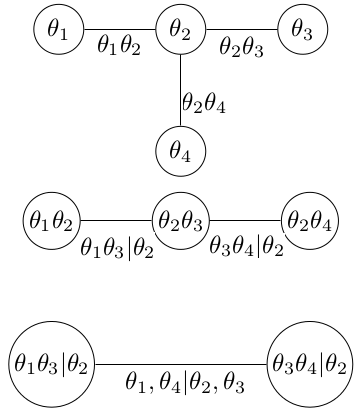
\includegraphics[width=0.4\linewidth,height=\textheight,keepaspectratio]{vines.png}
\vspace{2mm}
\caption{An example of a Vine Copula over four variables. The edges in the top tree represent unconditional bivariate copulae between the parameters on the connected nodes. The second tree edges represent the bivariate copulae for $\theta_1 \theta_3 | \theta_2$ and for $\theta_3 \theta_4 | \theta_2$, the conditioning on $\theta_2$ caused by its appearance in each connected node. The edge in the final tree represents the bivariate copula for $\theta_1, \theta_4 | \theta_2, \theta_3$, as both $\theta_2$ and $\theta_3$ appear in the connected nodes.}
\label{fig:vinecop}
\end{figure}

Denoting the number of elements in $\boldsymbol{\theta}$ by $k$, a vine copula for $q(\boldsymbol{\theta}, x_{0:T} | \boldsymbol{\lambda})$ contains $T+k$ trees, with a number of parameters included in $\boldsymbol{\lambda}$ that is $O(T+k)^2$. Constructing the vine so that the first $k$ trees do not contain copulae between any two elements of $x_t$ and the $k+1$'th tree contains copulae $c(x_t, x_{t+1} | \boldsymbol{\theta})$ will force trees $k+r$, with $r \geq 2$, to contain copulae $c(x_t, x_{t+r} | \boldsymbol{\theta}, x_{t+1:t+r-1})$. These can be set to the independence copula as the Markovian nature of the latent varables implies that $x_t$ and $x_{t+r}$ are conditionally independent given $\boldsymbol{\theta}$ and $x_{t+1:t+r-1}$, reducing the number of copula parameters to $O(Tk)$. For convenience the vine is further restricted so that, in each of the first $k$ trees, every $x_t$ has an edge to the same $\theta$ node with the same copula family. 

Di{\ss}mann's algorith (Di{\ss}mann, Brechmann, Czado and Kurowicka 2013) can be used to fit a vine copula to data, selecting both the set of edges for each tree and an appropriate copula family for each edge according to some criteria. A common critereon is to select the set of edges that maximise the sum of absolute empirical pairwise Kendall's Tau, with copula families that minimise AIC. This algorithm is modified to include the above restrictions. In the following, use of the letters $i$ and $j$ denote $\theta_i$ and $\theta_j$ and an alternative use of $t$ denotes $x_t$. Edges are denoted by $\{i, j | D \}$ and copula are given by $c(i, j | D)$ where $D$ is the conditioning set. Any copula that is to be included in the $q$ distribution is given by $\tilde{c}(i, j | D)$. Finally the empirical Kendall's Tau between a pair of variables is denoted by $\tau_{i, j | D}$. Noting that copulae are a function of the CDF of a random variable first transform all MCMC samples of $\boldsymbol{\theta}$ and $x_{0:T}$ to $(0, 1)$ using the empirical marginal CDFs. No restrictions are applied to the $\boldsymbol{\theta}$ sub-trees, so a $k$ dimensional vine for these parameters can be estimated using Di{\ss}mann's algorith by any critiera with selected edges $\{i, j | D\}$ and copulae $\tilde{c}(i, j | D)$ added to the first $k$ trees of the full vine. 

The first tree also contains edges from each $x_t$ to the same $\theta$ element, selected by calculating $\tau_{j, t}$ for each $\theta_j$ and $x_t$ and add edges $\{t, i^{(1)} \}$ where
\begin{equation}
\label{Vine:TauCrit}
i^{(1)} = \arg \underset{j}{\max} \sum_{t} \tau_{j, t}.
\end{equation}
For each copula family $m$ and each $t$, estimate the copula $c_m(i^{(1)}, t)$ and choose one family for all of these copula as $\tilde{c}(i^{(1)}, t)$. The decision could be on the basis of criteria such as `minimises the sum of AIC across $t$' or `minimises AIC for the most $t$'. In each tree $l = 2, \dots, k$ this processs is repeated: Calculate $\tau_{j, t | i^{(1)}, \dots, i^{(l-1)}}$ for each $t$ and element of $\theta$ that has an edge to $\theta^{(l-1)}$ in one of the first $l-1$ trees, then choose $\theta_{i^{(l)}}$ where
\begin{equation}
\label{Vine:TauCrit}
i^{(l)} = \arg \underset{j}{\max} \sum_{t} \tau_{j, t}.
\end{equation}
Estimate copulae $c_m(i^{(l)}, t | i^{(1:l-1)})$ for each $t$ and $m$ and select a family as $\tilde{c}(i^{(l)}, t |i^{(1:l-1)})$. Tree $k+1$ contains edges $\{t, t+1 |  i^{(1:k)} \}$, with an optimal copula family $\tilde{c}(t, t+1 |i^{(1:k)})$. Tree $k+r$ with $r > 1$ must then contain edges $\{t, t+r |  i^{(1:k)}, t+1, \dots, t+r-1 \}$ with $\tilde{c}(t, t+r |  i^{(1:k)}, t+1, \dots, t+r-1)$ chosen to be the independence copula. This approach is given in Algorithm \ref{alg:MIVB}.

The product of all $\tilde{c}$ copula and selected $\tilde{q}$ marginals forms the approximating distribution $q(\boldsymbol{\theta}, x_{0:T} | \boldsymbol{\lambda})$. As the marginal distributions and copula for $x_t$ are identical for each $t$ additional latent variables $x_{T+1:T+S}$ can easily be included to form $q(\boldsymbol{\theta}, x_{0:T+S} | \boldsymbol{\lambda})$. The ELBO can be maximised for this $q$ using Copula Variational Inference (Tran, Blei and Airoldi 2015). As we are interested in forecasts of $y_{T+S+h}$ and $x_t$ is Markovian, the distribution of each $x_t$ is irrelevant given the distribution of $x_s, s > t$. Holding $\lambda$ parameters assocaited with $x_t, t = 0, \dots, T$ fixed at MCMC data estimated values will drastically reduce the computational cost of the gradient ascent algorirhtm as only the $\lambda$ parameters associated with the marginal distributions of $\theta$ and $x_{T+1:T+S}$, as well as the copulae between these, needs to be optimised.

\begin{algorithm}[H]
 \SetKwInOut{Input}{Input}
 \Input{Observations of $\boldsymbol{\theta}, x_{1:T}$,  $k$, the number of elements in $\boldsymbol{\theta}$.}
 \KwResult{Set of copulae $\tilde{c}(\cdot, \cdot)$}
 Transform observations for each variable to $(0, 1)$ by the inverse CDF\;
 Apply Di{\ss}mann's algorithm to $\boldsymbol{\theta}$, denote the selected edges by $\{i, j | D \}_l$ and copulae by $\tilde{c}(i, j | D)_l$ where $D$ is the conditioning set for each copula and $l = 1, \dots, k-1$ is the tree. \;
 Calculate $\hat{\tau}_{j, t}$ for each $j$ and $t$ \;
 Find $i^{(1)} = \arg \underset{j}{\max} \sum_t \hat{\tau}_{j, t}$. \;
 Add edges $\{i, j |\}_1$ and $\{i^{(1)}, t \}$ to Tree $1$. \;
 For each $t$ and copula family $m$ estimate $c_m(i^{(1)}, t)$.\;
 Select $\tilde{c}(i^{(1)}, t)$.\;
 For each $\tilde{c}(i, j)_1$ calculate $\theta_i | \theta_j$ and $\theta_j | \theta_i$; transform to (0, 1).\;
 For each $t$ use $\tilde{c}(i^{(1)}, t)$ to calculate $x_t | \theta_{i^{(1)}}$; transform to (0, 1).\;
 \For {$l = 2, \dots, k$} {
    Calculate $\hat{\tau}_{j, t | i^{(1:l-1)}}$ for $x_t | \theta_{i^{(1:l-1)}}$ and each $\theta_j | D$ where $D$ matches the $x_t$ conditioning set $\theta_{i^{(1:l-1)}}$. \;
  Find $i^{(l)} = \arg \underset{j}{\max} \sum_t \hat{\tau}_{j, t | i^{(1:l-1)}}$. \;
  Add edges $\{i, j | D\}_l$ and $\{i^{(l)}, t |  i^{(1:l-1)}\}$ to Tree $l$. \;
  For each $t$ and copula family $m$ estimate $c_m(i^{(l)}, t |i^{(1:l-1)})$.\;
  Select $\tilde{c}(i^{(l)}, t |i^{(1:l-1)})$.\;
  For each $\tilde{c}(i, j | D)_l$ calculate $\theta_i | \theta_j, \theta_D$ and $\theta_j | \theta_i, \theta_D$; transform to (0, 1).\;
  For each $\tilde{c}(i^{(l)}, t |i^{(1:l-1)})$ calculate $x_t | \theta_{i^{(1:l)}}$; transform to (0, 1).\;
 }
  For each $t$ in $2, \dots, T$ and copula family $m$ estimate $c_m(t, t-1 | \boldsymbol{\theta}).$ \;
  Select $\tilde{c}(t, t-1 | \boldsymbol{\theta})$. \;
   \caption{MIVB Vine selection algorithm}
  \label{alg:MIVB}
\end{algorithm}

\section{Simulation Results}
\subsection{DLM}
\subsection{SVM}

\section{Empirical Application}

\section{Discussion}


\newpage
\section{Appendix}
\iffalse % hide entire appendix

\subsection{Variational Approximations for the Dynamic Linear Model}

The joint distribution $p(y_{1:T}, \boldsymbol{\theta}, x_{1:T})$ for the Dynamic Linear Model is given by

\begin{align}
p(y_{1:T}, \boldsymbol{\theta}, x_{1:T}) &= \prod_{t=1}^{T} \bigg( \mathcal{N}(y_t | x_t + \gamma, \sigma^2_y) \mathcal{N}(x_t | \phi x_{t-1}, \sigma^2_x) \bigg) \mathcal{N}(x_0 | 0, \sigma^2_x (1 - \phi^2)^{-1}) \nonumber \\
&\mathcal{N}(\gamma | \bar{\gamma}, \sigma^2_{\gamma}) \mathcal{U}(\phi | -1, 1) \mathcal{IG}(\sigma^2_y | \alpha_y, \beta_y)\mathcal{IG}(\sigma^2_x | \alpha_x, \beta_x) 
\end{align}
with 
\begin{align}
\ln(p(y_{1:T}, \boldsymbol{\theta}, x_{1:T})) &= -(T/2 + \alpha_y + 1) \ln(\sigma_y^2) -(T/2 + \alpha_x + 3/2) \ln(\sigma_x^2) \nonumber \\
&- \frac{\sum_{t=1}^{T}(y_t - \gamma - x_t)^2}{2 \sigma^2_y} - \frac{x_0^2(1 -\phi^2) + \sum_{t=1}^{T}(x_t - \phi x_{t-1})^2}{2 \sigma^2_x} \nonumber \\
&- \frac{(\gamma - \bar{\gamma})^2}{2 \sigma^2_{\gamma}} - \frac{\beta_y}{\sigma^2_y} - \frac{\beta_x}{\sigma^2_x} + c \label{logjoint}. 
\end{align}

We use Kingma and Welling's (2014) reparameterised approach to the variational approximation in all of our applications, with the transforms detailed in Sections 4.1.1 - 4.1.3.

\subsubsection{The Multivariate Normal Approximations}

The distribution $q(\boldsymbol{\theta}, x_{1:T} | \boldsymbol{\lambda})$ for the first two approaches is defined by the following transformation, where $\epsilon_{1}, \dots, \epsilon_{T+5}$ have independent standard normal distributions.
\begin{align}
\sigma^2_y &= \exp(\mu_1 + L_{11} \epsilon_1)  \label{transform1} \\
\sigma^2_x &= \exp(\mu_2 + L_{21} \epsilon_1 + L_{22} \epsilon_2) \label{transform2} \\
\phi &= \mu_3 + L_{31} \epsilon_1 + L_{32} \epsilon_2 + L_{33} \epsilon_3 \label{transform3} \\
\mu &= \mu_4 + L_{41} \epsilon_1 + L_{42} \epsilon_2 + L_{43} \epsilon_3 + L_{44} \epsilon_4 \label{transform4} \\
x_t &= \mu_{t+5} + \sum_{j=1}^{t+5} L_{t+5, j} \epsilon_j \mbox{ for } t = 0, \dots, T \label{transform5} 
\end{align}

The approximation is parameterised by $\boldsymbol{\lambda} = \{ \boldsymbol{\mu}, \textbf{L} \}$ where $\textbf{L}$ is the lower triangular decomposition of the Multivariate Normal variance matrices $\textbf{V}$ and $\boldsymbol{\Sigma}$. In the case where the diagonal matrix $\textbf{V}$ is used, restrict $L_{ij} = 0$ for $i \neq j$.
The log determinant of the Jacobian is given by
\begin{equation}
\label{logdetjac}
\ln(|J|) = \left(\sum_{i = 1}^{i = T+5} \ln(L_{ii}) + \mu_1 + L_{11} \epsilon_1 + \mu_2 + L_{21} \epsilon_1 + L_{22} \epsilon_2\right).  
\end{equation}

Derivatives of (\ref{logjoint}) with respect to $\boldsymbol{\theta}$ and $x_{0:T}$, as well as derivatives of (\ref{transform1}) - (\ref{logdetjac}) with respect to $\boldsymbol{\mu}$ and $\textbf{L}$ are easily obtained for use in estimating the gradient of the ELBO.

\subsubsection{Copula Approximation}

Di{\ss}mann's algorithm was applied to MCMC draws of $\boldsymbol{\theta} = \{ \sigma^2_y, \sigma^2_x, \phi, \gamma \}$ and $x_{0:T}$. The first tree was estimated via:
\begin{enumerate}
\item Map $\boldsymbol{\theta}, x_{0:T}$ to $(0, 1)^{T+5}$ by taking the empirical marginal CDF of each variable.
\item Calculate the absoluate value of Kendall's Tau, $|\tau_{ij}|$ for  $i, j = 1, \dots, T+5$ between each pair.
\item Find the maximum spanning tree by Kruskal's algorithm with edge weights given by $|\tau_{ij}|$, subject to the restrictions that no edge may be selected between two $x_t$ variables and each $x_t$ must have an edge to the same element of $\theta$. This tree forms $T_1$.
\end{enumerate}
The tree $T_1$ that was selected only permitted one vine factorisation for trees $T_2, \dots, T_k$ so a further application of Di{\ss}mann's algorithm was unneccesary. The full vine copula selected is shown in Figure (\ref{fig:dlmvinecop})

\begin{figure}[h]
\centering
\tikz{ %
    \node[latent] (x) {$x_{0:T}$} ; %
    \node[latent, right = of x] (gamma) {$\gamma$} ; %
    \node[latent, right = of gamma] (sigy) {$\sigma^2_y$} ; %
    \node[latent, right = of sigy] (sigx) {$\sigma^2_x$} ; %
    \node[latent, right = of sigx] (phi) {$\phi$} ; %
    \edge [-] {x} {gamma} ; %
    \edge [-] {gamma} {sigy} ; %
    \edge [-] {sigy} {sigx} ; %
    \edge [-] {sigx} {phi} ; %
    
    \node[latent, below = of x] (xgamma) {$x_{0:T}, \gamma$} ; %
    \node[latent, right = of xgamma] (gammasigy) {$\gamma, \sigma^2_y$} ; %
    \node[latent, right = of gammasigy] (sigysigx) {$\sigma^2_y, \sigma^2_x$} ; %
    \node[latent, right = of sigysigx] (sigxphi) {$\sigma^2_x, \phi$} ; %
    \edge [-] {xgamma} {gammasigy} ; %
    \edge [-] {gammasigy} {sigysigx} ; %
    \edge [-] {sigysigx} {sigxphi} ; %
    
    \node[latent, below = of xgamma] (xsigy) {$x_{0:T}, \sigma^2_y | \gamma$} ; %
    \node[latent, right = of xsigy] (gammasigx) {$\gamma, \sigma^2_x | \sigma^2_y$} ; %
    \node[latent, right = of gammasigx] (sigyphi) {$\sigma^2_y, \phi | \sigma^2_x$} ; %
    \edge [-] {xsigy} {gammasigx} ; %
    \edge [-] {gammasigx} {sigyphi} ; %
    
    \node[latent, below = of xsigy] (xsigx) {$x_{0:T}, \sigma^2_x | \sigma^2_y, \gamma$} ; %
    \node[latent, right = of xsigx] (gammaphi) {$\gamma, \phi | \sigma^2_x, \sigma^2_y$} ; %
    \edge [-] {xsigx} {gammaphi} ; %
    
    \node[latent, below = of xsigx] (x1) {$x_1, \phi | \gamma, \sigma^2_x, \sigma^2_y$} ; %
    \node[latent, left = of x1] (x0) {$x_0, \phi | \gamma, \sigma^2_x, \sigma^2_y$} ; %
    \node[latent, right = of x1] (dots) {$\dots$} ; %
    \node[latent, right = of dots] (xT1) {$x_{T-1}, \phi | \gamma, \sigma^2_x, \sigma^2_y$} ; %
    \node[latent, right = of xT1] (xT) {$x_T, \phi | \gamma, \sigma^2_x, \sigma^2_y$} ; %
    \edge [-] {x0} {x1} ; %
    \edge [-] {x1} {dots} ; %
    \edge [-] {dots} {xT1} ; %
    \edge [-] {xT1} {xT} ; %
    
    \node[latent, below = of x1] (x0x1) {$x_0, x_1 | \boldsymbol{\theta}$} ; %
    \node[latent, right = of x0x1] (x1x2) {$x_1, x_2 | \boldsymbol{\theta}$} ; %
    \node[latent, right = of x1x2] (dots2) {$\dots$} ; %
    \node[latent, right = of dots2] (xT1xT) {$x_{T-1}, x_T | \boldsymbol{\theta}$} ; %
    \edge [-] {x0x1} {x1x2} ; %
    \edge [-] {x1x2} {dots2} ; %
    \edge [-] {dots2} {xT1xT} ; %
}
\caption{The vine copula used for the Dynamic Linear Model. Each node containing $x_{0:T}$ denotes $T+1$ individual nodes connected to the same neighbouring node.}
\label{fig:dlmvinecop}
\end{figure}


\subsubsection{Algorithm Details}

Gradient Ascent is performed with the Adam optimiser from Kingma and Ba (2015). Adam uses estimates of the first two moments of the gradient, and is described in Algorithm (\ref{alg:adam}). We use $\alpha = 0.1, \beta_1 = 0.9, \beta_2 = 0.999$ and $\epsilon = 10^{-8}$.

\begin{algorithm}[H]
 \SetKwInOut{Input}{Input}
 \Input{Method to estimate gradients of $f(\lambda), \alpha, \beta_1, \beta_2, \epsilon$}
 \KwResult{Optimal Parameters $\lambda$}
 Set $m_0 = 0$\;
 Set $v_0 = 0$\;
 Set $t = 0$\;
 \While{not converged}{
  $t = t + 1$\;
  $g_t = \nabla_{\lambda}f(\lambda)$ \;
  $m_t = \beta_1 m_{t-1} + (1-\beta_1) g_t$ \;
  $v_t = \beta_2 v_{t-1} + (1-\beta_2) v_t$ \;
  $\hat{m}_t = m_t / (1 - \beta_1^t)$ \;
  $\hat{v}_t = v_t / (1 - \beta_2^t)$ \;
  $\lambda = \lambda + \alpha \cdot \hat{m}_t / (\sqrt{\hat{v}_t} + \epsilon)$
  }
 \caption{Adam Optimiser}
  \label{alg:adam}
\end{algorithm}

Increases in $N$, the number of simulations of the gradient of the ELBO per iteration, should increase the accuracy of the estimate and thus reduce the number of iterations required for convergence at a cost to compuation time per iteration. Figure (\ref{fig:RuntimeELBO}) plots the converged value of the ELBO against algorithm run time for a range of values of $N$. On this basis, we select $N = 5$ for the diagonal approximation and $N = 100$ for the non-diagonal approximation.

\begin{figure}[h]
\centering
\includegraphics{RuntimevELBO}
\caption{Converged ELBO value versus total runtime for a range of values of $N$ and approximation functional forms.}
\label{fig:RuntimeELBO}
\end{figure}
\fi

\end{document}
